%%%%%%%%%%%%%%%%%%%%%%%%%%%%%%%%%%%%%%%%%%%%%%%%%%%%%%%%%%%%%%%%%%%%%%%%%%%%%%%%%%
\begin{frame}[fragile]\frametitle{}
\begin{center}
{\Large Concepts}
\end{center}
\end{frame}



%%%%%%%%%%%%%%%%%%%%%%%%%%%%%%%%%%%%%%%%%%%%%%%%%%%%%%%%%%%
\begin{frame}[fragile]\frametitle{Overview}

Overview of traditional RAG and two typical GraphRAG workflows.

    \begin{itemize}
        \item Non-graph RAG organizes the corpus into chunks, ranks them by similarity, and retrieves the most relevant text for generating responses.
        \item Knowledge-based GraphRAG extracts detailed knowledge graphs from the corpus using entity recognition and relation extraction, offering fine-grained, domain-specific information.
        \item Index-based GraphRAG summarizes the corpus into high-level topic nodes, which are linked to form an index graph, while the fact linking maps topics to text.
    \end{itemize}
	
	{\tiny (Ref: Awesome-GraphRAG (GraphRAG Survey))}
	
\end{frame}

% %%%%%%%%%%%%%%%%%%%%%%%%%%%%%%%%%%%%%%%%%%%%%%%%%%%%%%%%%%%%%%%%%%%%%%%%%%%%%%%%%%
% \begin{frame}[fragile]\frametitle{}
% \begin{center}
% {\Large Knowledge Graphs}
% \end{center}
% \end{frame}

%%%%%%%%%%%%%%%%%%%%%%%%%%%%%%%%%%%%%%%%%%%%%%%%%%%%%%%%%%%
\begin{frame}[fragile]\frametitle{Btw, What is Knowledge Graph?}
    \begin{block}{Definition}
A Knowledge Graph is a structured way of representing 
information, typically using nodes and edges to depict 
relationships between entities (e.g., people, places, 
things, concepts). 
These entities and their interconnections form a 
graph-like structure, which can be used to model 
complex sets of data and the relationships within that 
data.
    \end{block}
	
	{\tiny (Ref: The GenAI Stack - Andreas Kollegger - Neo4j)}
	
\end{frame}


%%%%%%%%%%%%%%%%%%%%%%%%%%%%%%%%%%%%%%%%%%%%%%%%%%%%%%%%%%%
\begin{frame}[fragile]\frametitle{}

	\begin{center}
	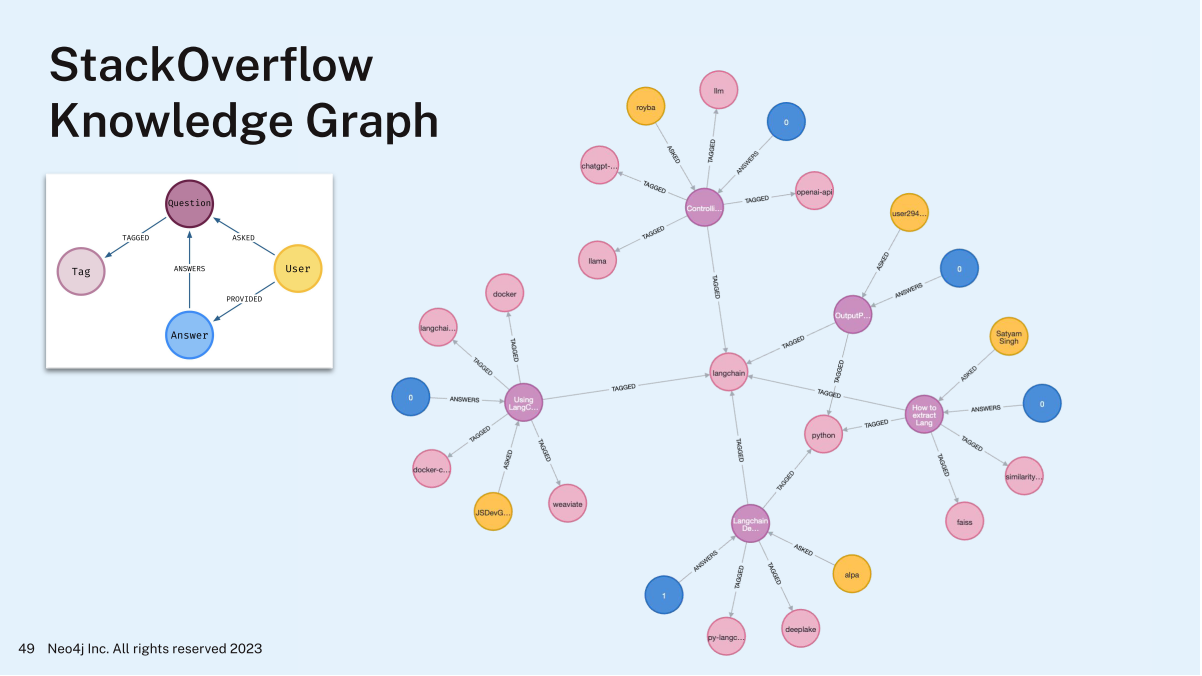
\includegraphics[width=\linewidth,keepaspectratio]{graphrag7}
	\end{center}
	
\end{frame}

% %%%%%%%%%%%%%%%%%%%%%%%%%%%%%%%%%%%%%%%%%%%%%%%%%%%%%%%%%%%
% \begin{frame}[fragile]\frametitle{}

	% \begin{center}
	% 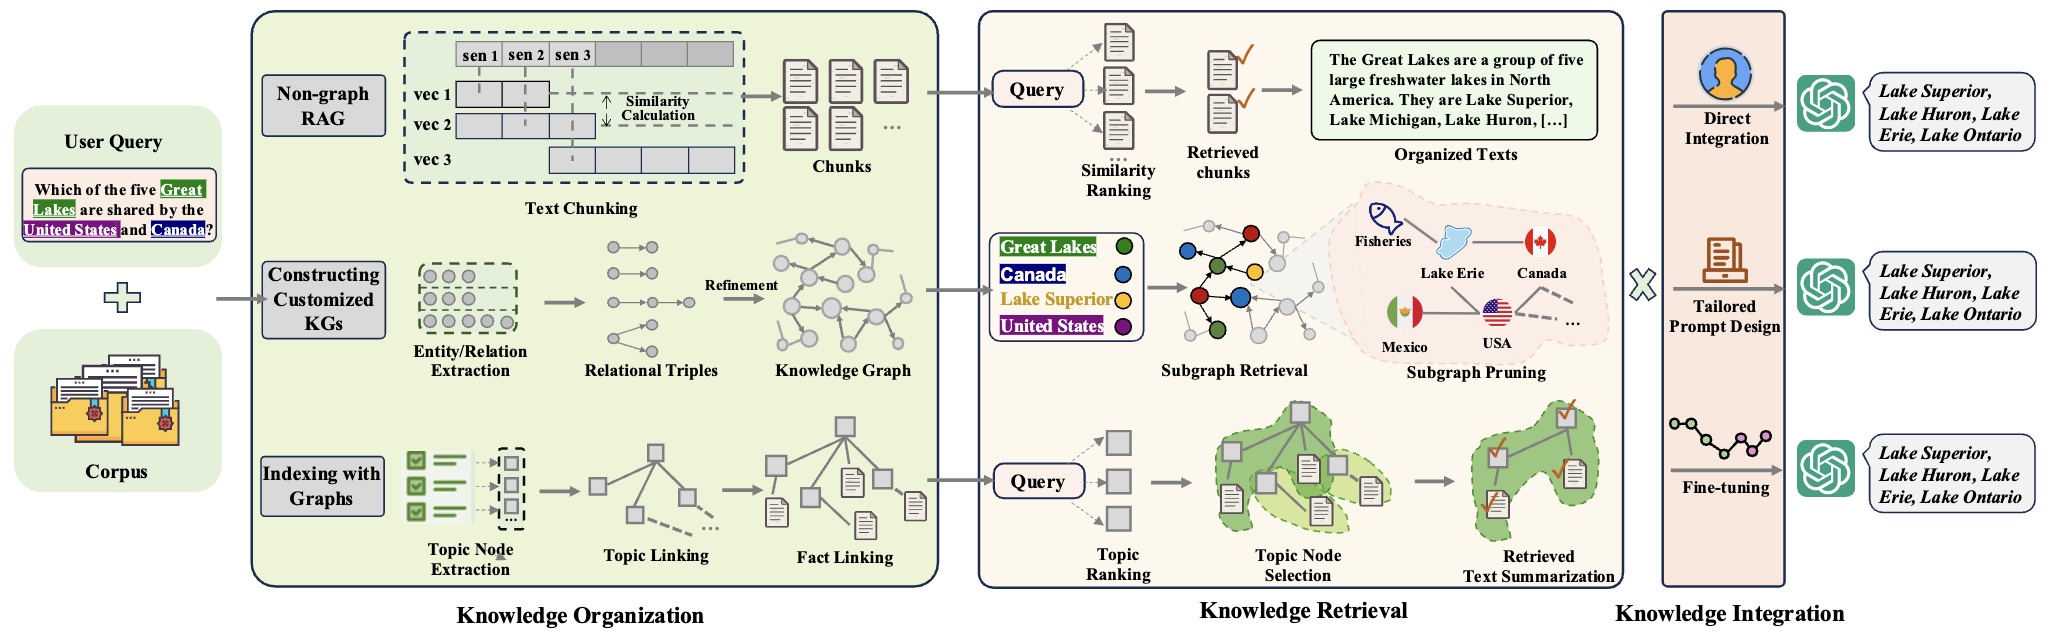
\includegraphics[width=\linewidth,keepaspectratio]{graphrag11}
	% \end{center}
	
% \end{frame}

%%%%%%%%%%%%%%%%%%%%%%%%%%%%%%%%%%%%%%%%%%%%%%%%%%%%%%%%%%%
\begin{frame}[fragile]\frametitle{Graph Construction Economy Principle}
    \begin{itemize}
        \item Complex graphs require significant computational resources.
        \item Trade-off: Performance gains must justify resource investment.
        \item Aim: Maximize performance-to-resource ratio.
    \end{itemize}
\end{frame}


%%%%%%%%%%%%%%%%%%%%%%%%%%%%%%%%%%%%%%%%%%%%%%%%%%%%%%%%%%%%%%%%%%%%%%%%%%%%%%%%%%
\begin{frame}[fragile]\frametitle{}
\begin{center}
{\Large Approaches}
\end{center}
\end{frame}

%%%%%%%%%%%%%%%%%%%%%%%%%%%%%%%%%%%%%%%%%%%%%%%%%%%%%%%%%%%
\begin{frame}[fragile]\frametitle{Cost-Efficient GraphRAG Approach}
    \begin{itemize}
        \item Leverages graphs for RAG without high costs.
        \item Minimizes reliance on LLMs or uses smaller on-premise models.
        \item Structured as a layered graph:
        \begin{itemize}
            \item Ontology Layer – Defines domain structure (fixed or nearly fixed).
            \item Document Layer – Contains chunked documents, similar to a vector DB.
            \item Entity Layer (Optional) – Extracted entities enhance search.
        \end{itemize}
    \end{itemize}
\end{frame}

%%%%%%%%%%%%%%%%%%%%%%%%%%%%%%%%%%%%%%%%%%%%%%%%%%%%%%%%%%%
\begin{frame}[fragile]\frametitle{Challenges in Ontology-Based Graphs}
    \begin{itemize}
        \item Not all datasets belong to a well-defined domain.
        \item Subject Matter Experts (SMEs) may not be available.
        \item Eliminating fixed ontology layer could improve flexibility.
    \end{itemize}
\end{frame}

%%%%%%%%%%%%%%%%%%%%%%%%%%%%%%%%%%%%%%%%%%%%%%%%%%%%%%%%%%%
\begin{frame}[fragile]\frametitle{NLP-Powered Graph Approach}
    \begin{itemize}
        \item Drops the ontology layer for cost-efficiency.
        \item Graph consists of:
        \begin{itemize}
            \item Document Layer – Contains document chunks.
            \item Tokens Layer – Extracted tokens improve search.
        \end{itemize}
        \item NLP reduces dependency on LLMs.
    \end{itemize}
\end{frame}

%%%%%%%%%%%%%%%%%%%%%%%%%%%%%%%%%%%%%%%%%%%%%%%%%%%%%%%%%%%
\begin{frame}[fragile]\frametitle{Data Preprocessing Pipeline}
    \begin{itemize}
        \item Chunking – Splitting documents into segments.
        \item Embedding – Using Hugging Face model for embeddings.
        \item Graph Construction – Built using NetworkX or Neo4j.
        \item Token Extraction – Generates token, bigram, and trigram nodes.
    \end{itemize}
\end{frame}

%%%%%%%%%%%%%%%%%%%%%%%%%%%%%%%%%%%%%%%%%%%%%%%%%%%%%%%%%%%
\begin{frame}[fragile]\frametitle{Indexing and Interconnectivity}
    \begin{itemize}
        \item Tokens are shared across documents, interlinking content.
        \item Need to connect entities using context, logic, and semantics.
        \item Avoid reliance on massive models due to cost constraints.
    \end{itemize}
\end{frame}

%%%%%%%%%%%%%%%%%%%%%%%%%%%%%%%%%%%%%%%%%%%%%%%%%%%%%%%%%%%
\begin{frame}[fragile]\frametitle{Triple Extraction for Graph Optimization}
    \begin{itemize}
        \item Triple extraction improves retrieval efficiency.
        \item Uses a smaller transformer model fine-tuned for this task.
        \item Triplets mapped to token nodes enhance query performance.
        \item Queries traverse graph using triplet relationships.
    \end{itemize}
\end{frame}

%%%%%%%%%%%%%%%%%%%%%%%%%%%%%%%%%%%%%%%%%%%%%%%%%%%%%%%%%%%
\begin{frame}[fragile]\frametitle{Optimizing Graph-Based Retrieval}
    \begin{itemize}
        \item Combines standard RAG with triplet-enhanced retrieval.
        \item Retrieves relevant text chunks and connected triplets.
        \item Improves search relevance and reduces retrieval complexity.
    \end{itemize}
\end{frame}




%%%%%%%%%%%%%%%%%%%%%%%%%%%%%%%%%%%%%%%%%%%%%%%%%%%%%%%%%%%
\begin{frame}[fragile]\frametitle{}

	\begin{center}
	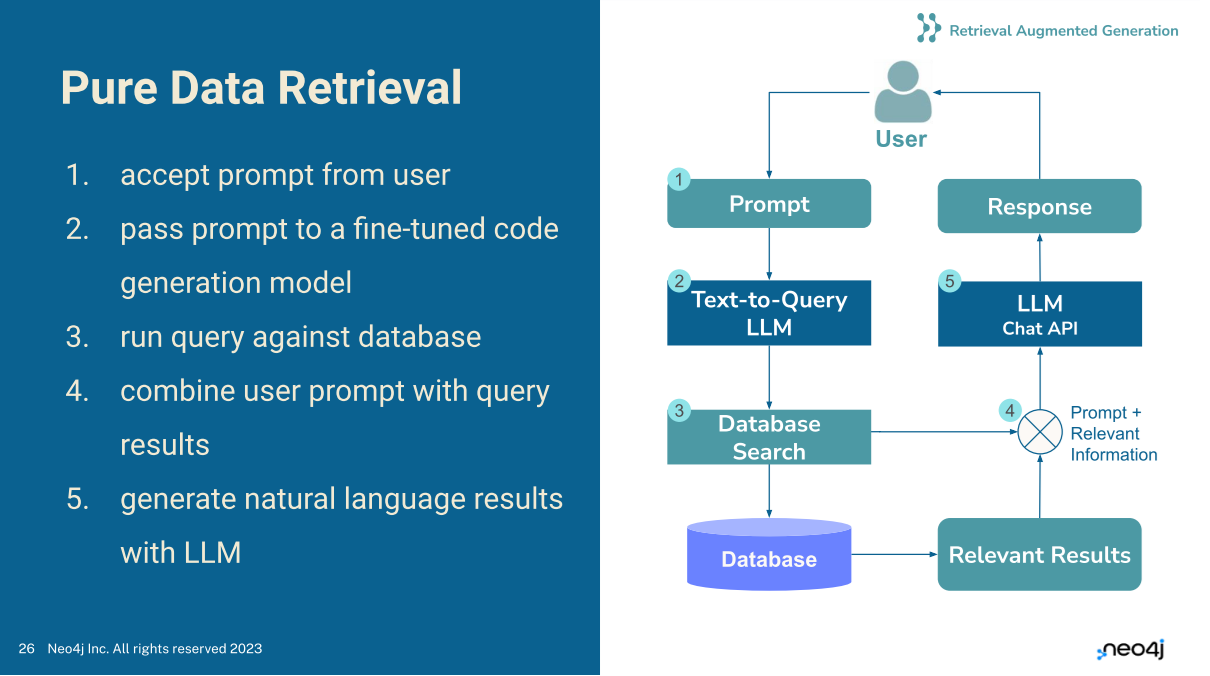
\includegraphics[width=\linewidth,keepaspectratio]{graphrag3}
	\end{center}
	
	
\end{frame}

%%%%%%%%%%%%%%%%%%%%%%%%%%%%%%%%%%%%%%%%%%%%%%%%%%%%%%%%%%%
\begin{frame}[fragile]\frametitle{Challenges}
    \begin{itemize}
        \item Getting it to work at all – generating syntactically correct queries
        \item Getting it to do the right thing – producing meaningful results
        \item Avoiding accidents – mistaken deletion
        \item Preventing malicious intent – SQL injection gone wild
    \end{itemize}
	
	{\tiny (Ref: The GenAI Stack - Andreas Kollegger - Neo4j)}
	
\end{frame}


%%%%%%%%%%%%%%%%%%%%%%%%%%%%%%%%%%%%%%%%%%%%%%%%%%%%%%%%%%%
\begin{frame}[fragile]\frametitle{}

	\begin{center}
	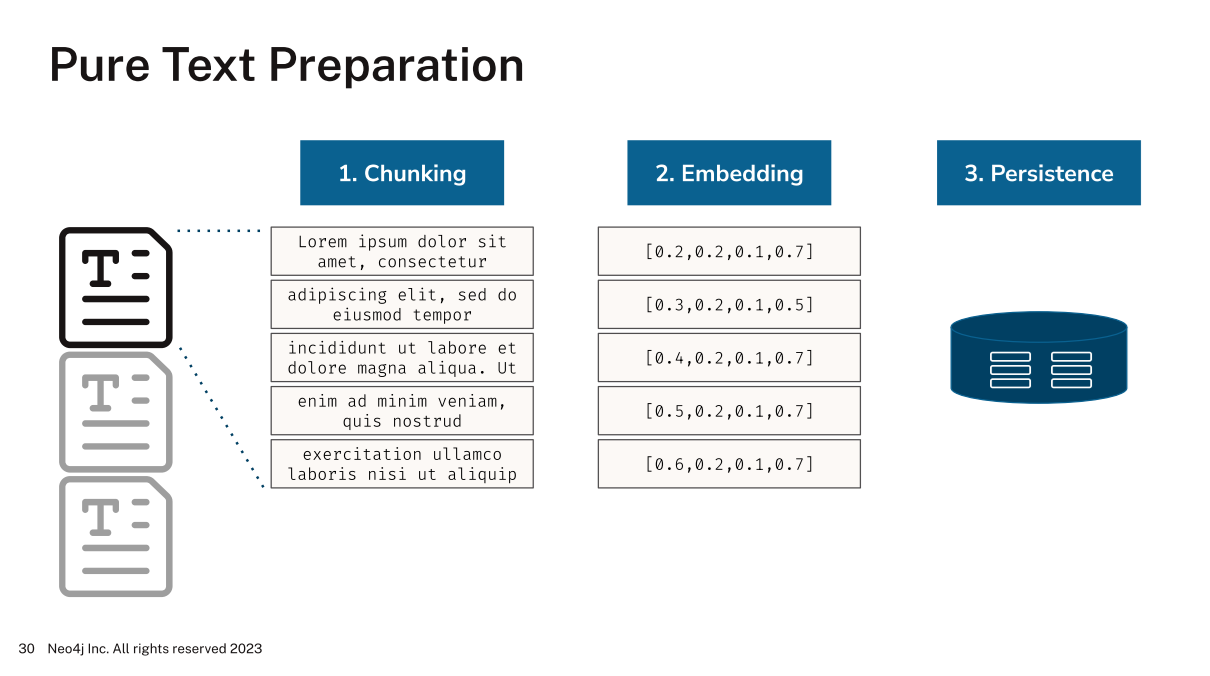
\includegraphics[width=\linewidth,keepaspectratio]{graphrag4}
	\end{center}
	
\end{frame}

%%%%%%%%%%%%%%%%%%%%%%%%%%%%%%%%%%%%%%%%%%%%%%%%%%%%%%%%%%%
\begin{frame}[fragile]\frametitle{Challenges}
    \begin{itemize}
        \item How?
		    \begin{itemize}
				\item pick a chunk method \& size
				\item each chunk is a record
				\item store chunk with metadata
				\item connect each chunk to original document
				\item connect previous/next chunk
		    \end{itemize}
        \item Challenges:
		    \begin{itemize}
				\item what makes a good chunk?
				\item potential chunk duplication
				\item how to re-assemble chunk context?
				\item  what about cross-document chunks?
				\item explaining the relevance
		    \end{itemize}
    \end{itemize}
	
	{\tiny (Ref: The GenAI Stack - Andreas Kollegger - Neo4j)}
	
\end{frame}

%%%%%%%%%%%%%%%%%%%%%%%%%%%%%%%%%%%%%%%%%%%%%%%%%%%%%%%%%%%
\begin{frame}[fragile]\frametitle{}

	\begin{center}
	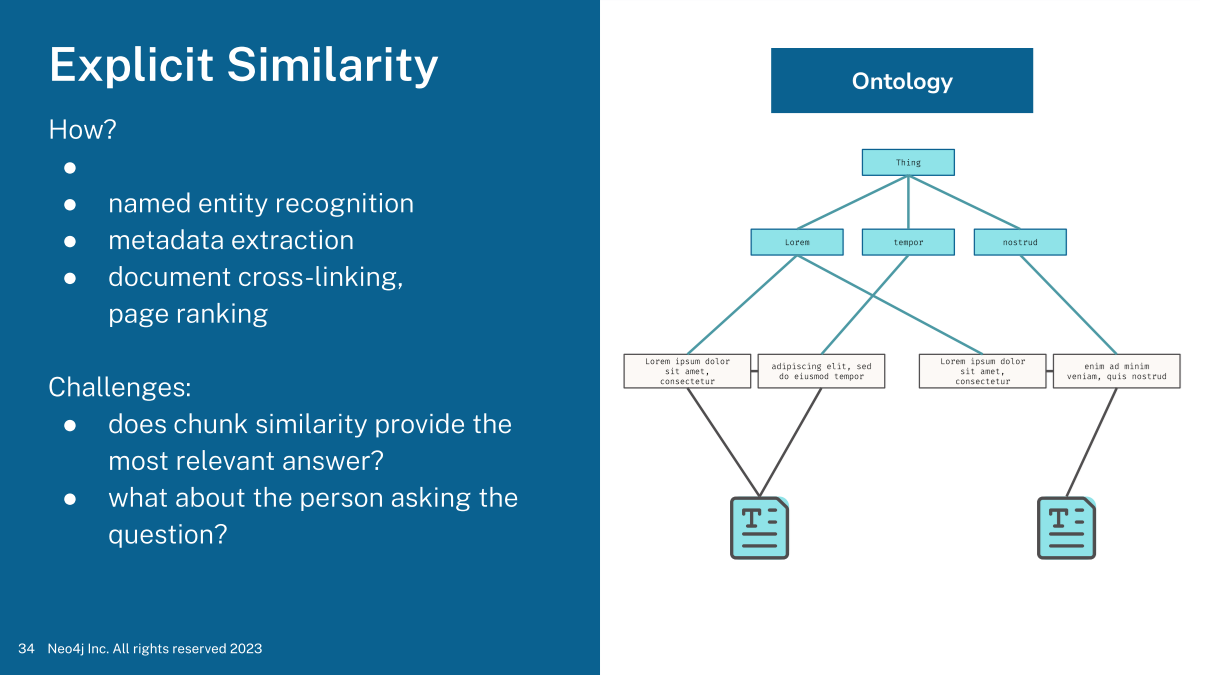
\includegraphics[width=\linewidth,keepaspectratio]{graphrag5}
	\end{center}
	
\end{frame}

%%%%%%%%%%%%%%%%%%%%%%%%%%%%%%%%%%%%%%%%%%%%%%%%%%%%%%%%%%%
\begin{frame}[fragile]\frametitle{}

	\begin{center}
	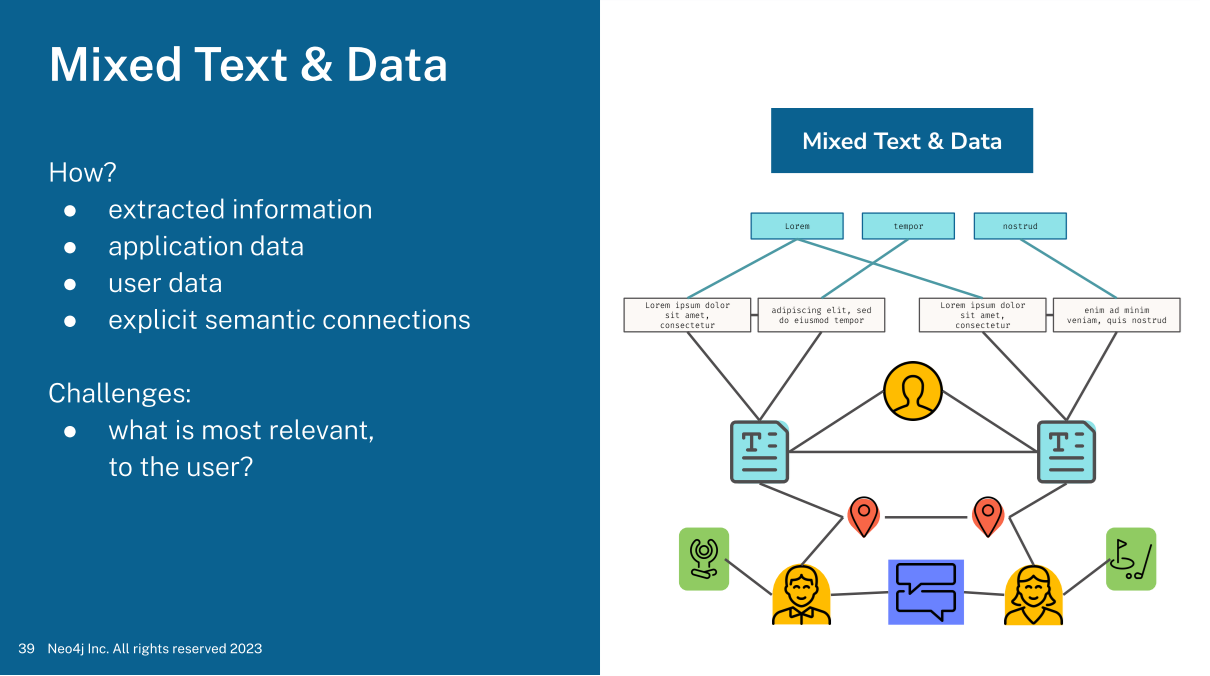
\includegraphics[width=\linewidth,keepaspectratio]{graphrag6}
	\end{center}
	
\end{frame}





% %%%%%%%%%%%%%%%%%%%%%%%%%%%%%%%%%%%%%%%%%%%%%%%%%%%%%%%%%%%
% \begin{frame}[fragile]\frametitle{}

	% \begin{center}
	% 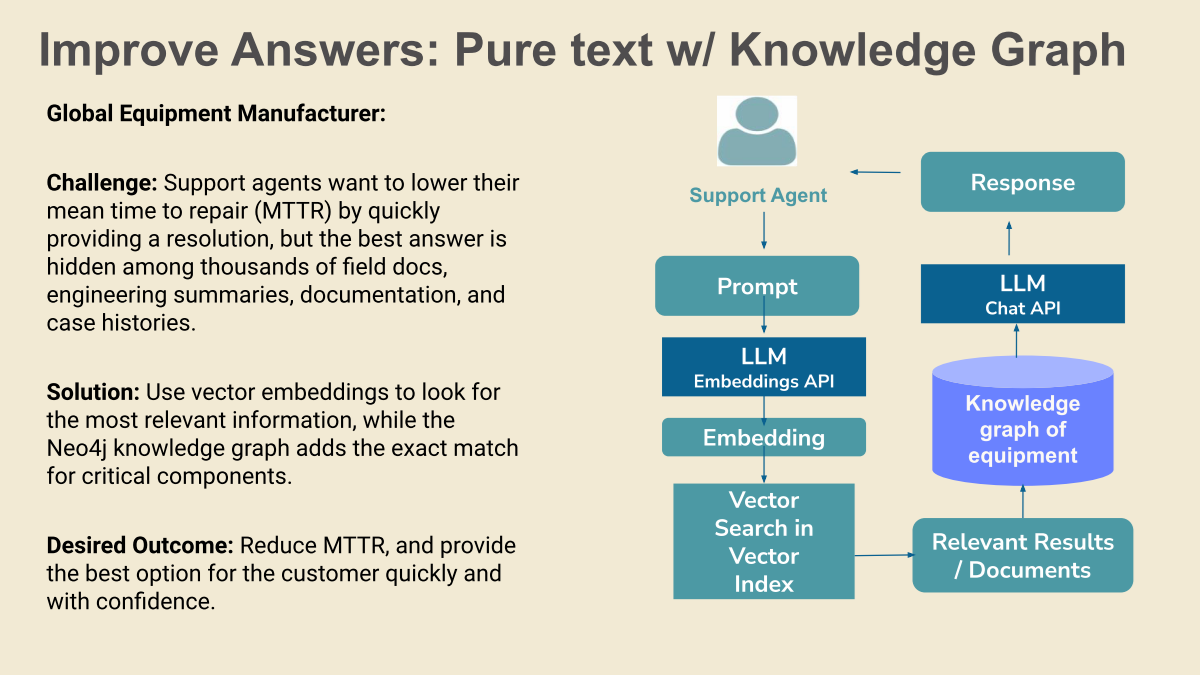
\includegraphics[width=\linewidth,keepaspectratio]{graphrag8}
	% \end{center}
	
% \end{frame}


% %%%%%%%%%%%%%%%%%%%%%%%%%%%%%%%%%%%%%%%%%%%%%%%%%%%%%%%%%%%
% \begin{frame}[fragile]\frametitle{}

	% \begin{center}
	% 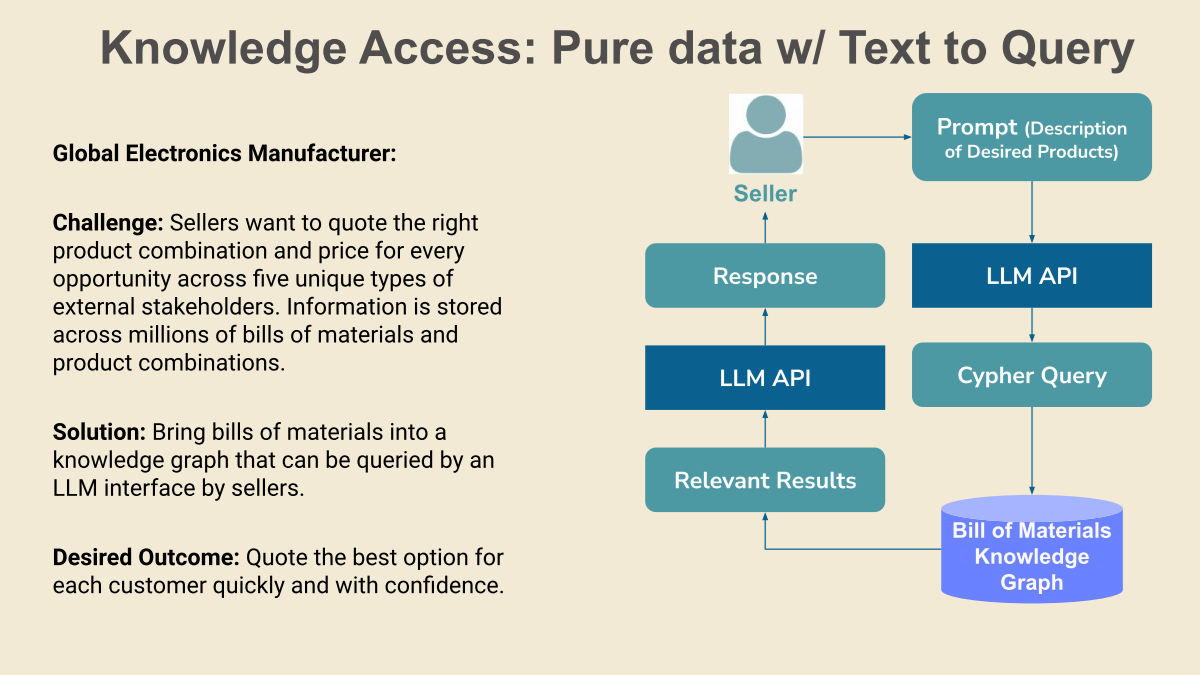
\includegraphics[width=\linewidth,keepaspectratio]{graphrag9}
	% \end{center}
	
% \end{frame}

% %%%%%%%%%%%%%%%%%%%%%%%%%%%%%%%%%%%%%%%%%%%%%%%%%%%%%%%%%%%
% \begin{frame}[fragile]\frametitle{}

	% \begin{center}
	% 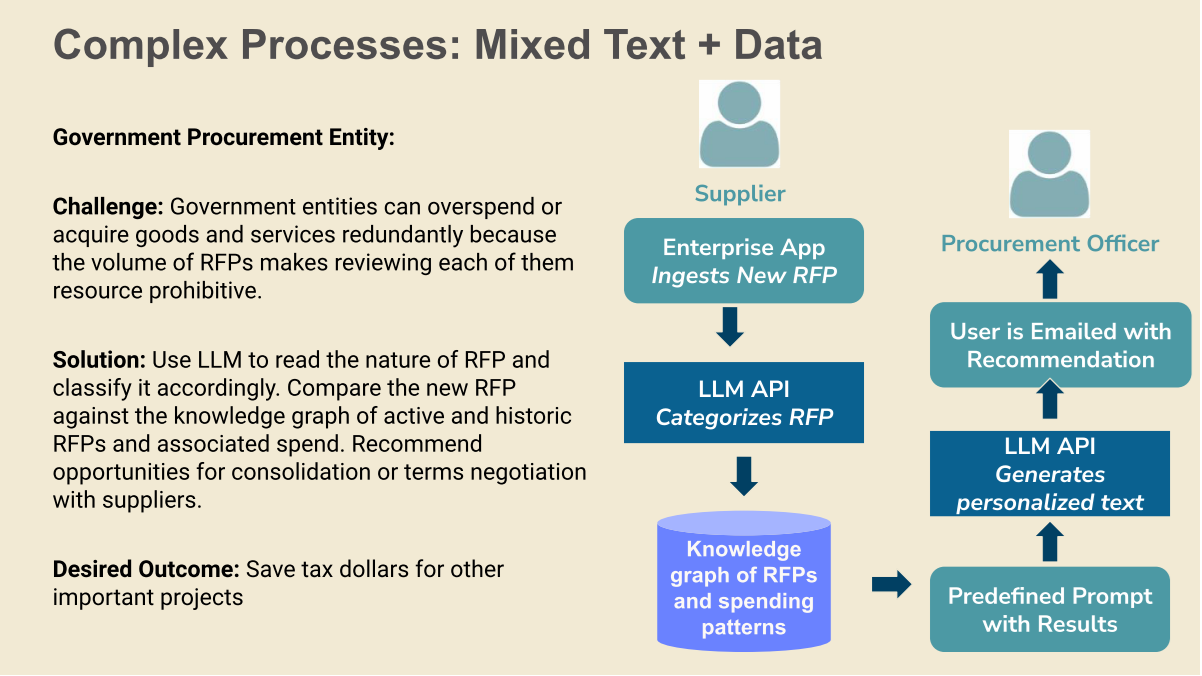
\includegraphics[width=\linewidth,keepaspectratio]{graphrag10}
	% \end{center}
	
% \end{frame}


%%%%%%%%%%%%%%%%%%%%%%%%%%%%%%%%%%%%%%%%%%%%%%%%%%%%%%%%%%%
\begin{frame}[fragile]\frametitle{Conclusion}
    \begin{itemize}
        \item GraphRAG scales from local to global knowledge representation.
        \item Community-based summaries improve response quality.
        \item Enables optimized retrieval with hierarchical partitioning.
    \end{itemize}
\end{frame}







